\section{Redes y Protocolos Particulares}
	\subsection{Frame Relay}
		\subsubsection{Introducción}
			\indent Frame Relay es un protocolo orientado a la conexión implementado, por lo general, en redes WAN. El mismo permite crear
			conexiones punto a punto en redes públicas a través de la creación de circuitos virtuales. Un circuito virtual consiste
			en un camino que se crea desde las terminales desde las cuales acceden los usuarios interesados en comunicarse 
			(DTE - Data Terminal Equipment) a partir de conmutadores que existen en la red Frame-Relay. Estos conmutadores, llamados DCEs 
			(Data Circuit-Terminating Equipment), consisten en equipos que multiplexan los paquetes que llegan de forma que los mismos arriben a destino. \\
			Existen dos tipos de circuitos virtuales que pueden crearse:

			\begin{itemize}
				\item PVCs (Permanent Virtual Circuits) 
				\item SVCs (Switched Virtual Circuits)
			\end{itemize} 

			Los PVCs consisten en circuitos virtuales fijos y son los que se utilizan en su mayoría. Sin embargo, Frame-Relay tiene soporte para crear
			SVCs, que son circuitos virtuales que se crean sólo cuando dos usuarios desean comunicarse y luego se destruyen al terminar la comunicación.
			Esto permite que los puertos de los DCEs puedan reutilizarse paras satisfacer la demanda de otros usuarios. Los SVCs, si bien son imprescindibles
			en redes como la telefonía, no encajan en un modelo de red como Internet debido a que la demanda por parte de los clientes es mayor y totalmente
			aleatoria. \\
			\indent Frame-Relay envía la información a través de los circuitos virtuales a través de paquetes (se dice que es una red que implementa la
			metodología de \textit{Packet Switching}). Los DCEs pueden identificar a donde deben ser dirigidos los paquetes a partir de su DLCI (Data Link 
			Connection Identifier) que no es más que un identificador de circuito virtual. Estos identificadores son locales, por lo cual dos redes 
			Frame-Relay pueden usar el mismo identificador sin problemas. 

		\subsubsection{Implementación}
			\indent En la topología presentada, los routers R1, R8, R9 y R15 se encuentran conectados a una \textit{nube} Frame Relay. Debido a que no se especifica
			como deben ser las conexiones entre los routers, se implementa una topología de malla completa de forma que todos los routers se encuentren conectados
			entre sí. En la tabla \ref{tab002} se exhiben las subredes asignadas a cada uno de estos enlaces. En la tabla \ref{tabFr001} se exhiben los DLCIs 
			asignados para cada uno de los circuitos virtuales creados. Cabe destacar que para que las conexiones punto a punto sean full-duplex, se crearon dos 
			circuitos virtuales para cada subred: uno para la ida de paquetes y otro para la vuelta de los mismos. En la figura \ref{figFr001} se exhibe un diagrama 	
			simplificado de como queda implementada la red Frame-Relay. 

			\begin{table}[!htbp]
				\centering
				\begin{tabular}{|c|c|c|}
					\hline
					Origen & DLCI & Destino	\\	
					\hline
					R1 & 108 & R8 \\
					\hline
					R8 & 801 & R1 \\
					\hline
					R1 & 109 & R9 \\
					\hline
					R9 & 901 & R1 \\
					\hline
					R1 & 105 & R15 \\	
					\hline 
					R15 & 501 & R1 \\
					\hline
					R8 & 809 & R9 \\
					\hline
					R9 & 908 & R8 \\
					\hline
					R8 & 805 & R15 \\
					\hline 
					R15 & 508 & R8 \\
					\hline
					R9 & 905 & R15 \\
					\hline
					R15 & 509 & R9 \\
					\hline
				\end{tabular}
				\caption{DLCIs correspondientes a cada circuito virtual}
				\label{tabFr001}
			\end{table}
 
			\begin{figure}[!htbp]
      	\centering
      	\begin{center}
      	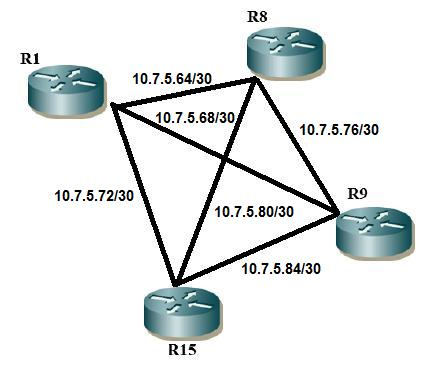
\includegraphics[width=0.8\textwidth]{Imagenes/framerelay1.jpg}
      	\end{center}
      	\captionof{figure}{Diagrama Frame Relay}
      	\label{figFr001}
			\end{figure}

			Para confeccionar la red Frame-Relay en el gns3 se utilizó el dispositivo \textit{FrameRelay-Switch}. El mismo permite configurar de forma amigable
			a través de un entorno GUI el enrutamiento de los paquetes que llegan al mismo a partir de los DLCIs. Con este dispositivo configurado, 
			sólo basta configurar las interfaces de los routers involucrados en la nube Frame-Relay para dejar operativa a la misma. \\
			\indent  Las interfaces que están conectadas a la red Frame-Relay deben ser interfaces Seriales (esto se debe a que los DTEs envían y reciben información
			a través del protocolo RS-232). Se debe especificar por la interfaz que salen los paquetes que los mismos deben ser encapsulados por medio de Frame-Relay. 
			Luego, como solo existe un enlace serial entre cada router y la nube, se implementan interfaces virtuales para cada uno de los enlaces punto a punto entre
			los routers. En cada uno de estos enlaces debe determinarse con que DLCI serán enviados los paquetes salientes de cada una de las interfaces. 
			A continuación, se exhibe la configuración pertinente a Frame-Relay implementada en cada uno de los routers conectados a la nube: \\

			\textbf{R1:}
			\begin{verbatim}
				interface Serial1/0
				no ip address
				encapsulation frame-relay
				
				interface Serial1/0.1 point-to-point
				ip address 10.7.5.65 255.255.255.252
				frame-relay interface-dlci 108

				interface Serial1/0.2 point-to-point
				ip address 10.7.5.69 255.255.255.252
				frame-relay interface-dlci 109

				interface Serial1/0.3 point-to-point
				ip address 10.7.5.73 255.255.255.252
				frame-relay interface-dlci 105
			\end{verbatim}	

			\vspace{0.5cm}
			\textbf{R8:}
			\begin{verbatim}
				interface Serial1/0
				no ip address
				encapsulation frame-relay

				interface Serial1/0.1 point-to-point
				ip address 10.7.5.66 255.255.255.252
				frame-relay interface-dlci 801

				interface Serial1/0.2 point-to-point
				ip address 10.7.5.77 255.255.255.252
				frame-relay interface-dlci 809

				interface Serial1/0.3 point-to-point
				ip address 10.7.5.81 255.255.255.252
				frame-relay interface-dlci 805
			\end{verbatim}	
			
			\vspace{0.5cm}
			\textbf{R9:}
			\begin{verbatim}
				interface Serial1/0
				no ip address
				encapsulation frame-relay

				interface Serial1/0.1 point-to-point
				ip address 10.7.5.70 255.255.255.252
				frame-relay interface-dlci 901

				interface Serial1/0.2 point-to-point
				ip address 10.7.5.78 255.255.255.252
				frame-relay interface-dlci 908

				interface Serial1/0.3 point-to-point
				ip address 10.7.5.85 255.255.255.252
				frame-relay interface-dlci 905
			\end{verbatim}	

			\vspace{0.5cm}
			\textbf{R15:}
			\begin{verbatim}
				interface Serial1/0
				no ip address
				encapsulation frame-relay

				interface Serial1/0.1 point-to-point
				ip address 10.7.5.74 255.255.255.252
				frame-relay interface-dlci 501

				interface Serial1/0.2 point-to-point
				ip address 10.7.5.82 255.255.255.252
				frame-relay interface-dlci 508

				interface Serial1/0.3 point-to-point
				ip address 10.7.5.86 255.255.255.252
				frame-relay interface-dlci 509
			\end{verbatim}
	

	\vspace{0.5cm}	
	\subsection{Tunnel GRE}
		\indent	Utilizando el tutorial expuesto en la cátedra, se creó un Tunnel GRE para encapsular en la red las conexiones de los routers R7 y R13 a Internet. 
		En la tabla \ref{tab002} se exhiben, entre otros, los datos de las subredes involucradas en el Tunnel. En la figura \ref{figGRE001} se exhibe 
		el equivalente de la topología luego de implementar el Tunnel. Gracias al mismo, se crea una conexión punto a punto entre R7 y R13, de forma que las 
		subredes \textit{Kentia} y \textit{Ulmaria} no son vistas en la red.
			\begin{figure}[!htbp]
    	  \centering
     	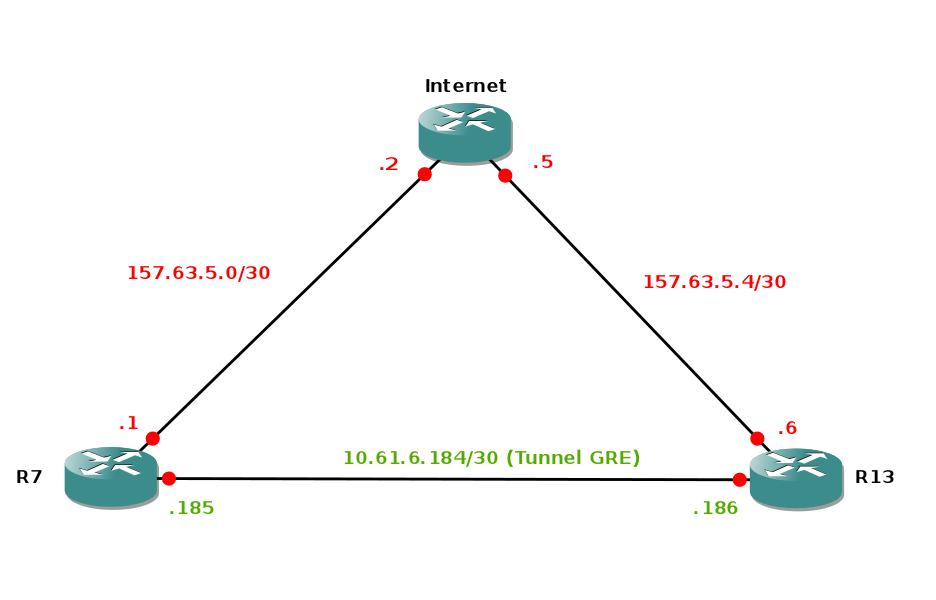
\includegraphics[width=12cm]{Imagenes/tunnelGRE.jpg}
     	 \captionof{figure}{Diagrama Tunnel GRE}
      	\label{figGRE001}
			\end{figure}

		Se exhibe a continuación, la configuración pertinente al protocolo GRE en los routers R7 y R13. Además de la configuración expuesta en el tutorial, se debe
		configurar de forma estática la comunicación de R7 a R13 y R13 a R7 a través de internet. De no especificarse esto, el Tunnel no se puede formar dado que 
		el protocolo no conoce como hacer para llegar desde un router, es decir, no saben que la comunicación entre R7 y R13 se realiza a través del router que
		simboliza Internet.  \\

		\textbf{R7:}
		\begin{verbatim}
			interface tunnel 10
			ip address 10.61.6.185 255.255.255.252
			tunnel source 157.63.5.1
			tunnel destination 157.63.5.6
			ip route 157.63.5.4 	255.255.255.252 	157.63.5.2
		\end{verbatim}

		\vspace{0.5cm}
		\textbf{R13:}
		\begin{verbatim}
			interface tunnel 20
			ip address 10.61.6.186 255.255.255.252
			tunnel source 157.63.5.6
			tunnel destination 157.63.5.1
			ip route 157.63.5.0 	255.255.255.252 	157.63.5.5
		\end{verbatim}	

	\vspace{0.5cm}	
	\subsection{VRRP - Virtual Router Redundancy Protocol}
		Vrrp es un protocolo de redundancia definido en el RFC 3768. El objetivo de vrrp es
		mantenter disponible una puerta de enlace para una determinada red. Para ello se
		define un router virtual y se configuran dos o más routers fisicos, de los cuales 
		solo uno va a realizar realmente el enrutamiento. Si el router fisíco falla o 
		alguna de sus interfaces (sobre las cuales se aplica el protocolo) cae, se negocia
		mediante el transpaso de mensajes quien es el próximo router que toma el rol de 
		maestro.\\
		En el caso del presente trabajo, se aplicó vrrp en dos pares de routers, por un 
		lado se aplicó a los routers R3 y R4, los cuales tienen en común la red A, y por
		el otro se aplicó a los routers R5 y R6 los cuales tienen interfaces en las redes 
		L y B.\\
		A continuación se muestra como se aplicó el protocolo en ambos casos.
		
		\subsubsection{Redundancia R3/R4}
			\textbf{R3:}
			En el caso de R3 se definió un tracking object que sensara la interface
			Ethernet0/2, correspondiente a la red A, y luego se configuró 
			dicha interface con los parametros de vrrp, se le asigno una prioridad de
			110, se definió la ip virtual 192.168.25.6. Por último se definió un 
			intervalo de 15 segundos para el intercambio de mensajes y un decremento 
			de 20 para la prioridad, según lo indique el tracking object.
			\begin{verbatim}
				hostname R3

				track 1 interface Ethernet0/2 ip routing

				interface Ethernet0/2
				ip address 192.168.25.4 255.255.255.0
				vrrp 12 description vrrp_lan_1
				vrrp 12 priority 110
				vrrp 12 timers advertise 15
				vrrp 12 timers learn
				vrrp 12 ip 192.168.25.6
				vrrp 12 track 1 decrement 20
			\end{verbatim}

			\textbf{R4:}
			En R4 no es necesario el tracking object, por lo que solo se configuraron
			los parametros correspondientes a vrrp mencionados anteriormente.
			\begin{verbatim}
				hostname R4

				interface ethernet0/2
				ip address 192.168.25.5 255.255.255.0
				vrrp 12 description vrrp_lan_3
				vrrp 12 priority 100
				vrrp 12 timers advertise 15
				vrrp 12 timers learn
				vrrp 12 ip 192.168.25.6
			\end{verbatim}

		\subsubsection{Redundancia R5/R6}
			\textbf{R5:}
			Tanto para R5 como para R6, se configuraron dos de las interfaces de los
			routers, puesto que son dos redes las que tienen en común (B y L). A la
			interface Ethernet0/0 correspondiente a la red L, se le configuró vrrp 10
			con ip virtual 10.61.6.196 y prioridad 100, mientras que a la interface 
			Ethernet0/1 correspondiente a la red B, se le configuro vrrp 11 con ip 
			virtual 10.111.25.196 y la misma prioridad.
			\begin{verbatim}
				hostname R5

				interface Ethernet0/0
				ip address 10.61.6.194 255.255.255.224
				vrrp 10 description vrrp_lan_1
				vrrp 10 priority 100
				vrrp 10 timers advertise 15
				vrrp 10 timers learn
				vrrp 10 ip 10.61.6.196

				interface Ethernet0/1
				ip address 10.111.25.194 255.255.255.192
				vrrp 11 description vrrp_lan_2
				vrrp 11 priority 100
				vrrp 11 timers advertise 15
				vrrp 11 timers learn
				vrrp 11 ip 10.111.25.196
			\end{verbatim}

			\textbf{R6:}
			Al igual que el caso anterior, en R6 se configuraron dos interfaces, y 
			ademas se definieron dos tracking objects qhe sensaran dichas interfaces. 
			Por un lado se definió el tracking object 1 sobre la interface Ethernet0/1
			en la cual se aplica vrrp 10, con ip virtual 10.61.6.196 como se mencionó
			anteriormente y prioridad 110. El segundo tracking object se aplicó sobre
			la interface Ethernet0/2 en la cual se definió vrrp 11, con ip virtual 
			10.111.25.196 y prioridad 110 (al igual que antes). La diferencia sustancial
			con la configuración de R3 y R4, es que en este caso, por mas que falle una
			de las dos inerfaces, se le decrementa la prioridad a ambas.
			\begin{verbatim}
				hostname R6

				track 1 interface Ethernet0/1 ip routing
				track 2 interface Ethernet0/2 ip routing

				interface Ethernet0/1
				ip address 10.61.6.195 255.255.255.224
				vrrp 10 description vrrp_lan_1
				vrrp 10 priority 110
				vrrp 10 timers advertise 15
				vrrp 10 timers learn
				vrrp 10 ip 10.61.6.196
				vrrp 10 track 1 decrement 20
				vrrp 10 track 2 decrement 20

				interface Ethernet0/2
				ip address 10.111.25.193 255.255.255.192
				vrrp 11 description vrrp_lan_2
				vrrp 11 priority 110
				vrrp 11 timers advertise 15
				vrrp 11 timers learn
				vrrp 11 ip 10.111.25.196
				vrrp 11 track 1 decrement 20
				vrrp 11 track 2 decrement 20
			\end{verbatim}